\documentclass[11pt,table,final,xcolor={usenames,dvipsnames,table}]{beamer}
\usetheme[]{Frankfurt}


\usepackage{listings}
\usepackage{multimedia} % Movies
\usepackage{fancyvrb,relsize}
\usepackage{commath}
\usepackage{graphicx}
\usepackage{array}
\usepackage{longtable}
\usepackage{algpseudocode} 
\usepackage{multirow}
\usepackage[math]{iwona}
\usepackage{wasysym}
% \usepackage[fleqn]{amsmath}
\usepackage{amssymb}
\usepackage{siunitx}
\usepackage{tikz} % Drawing
\usepackage{pgfplots}
\usepackage{pgfplotstable}
% \usepackage{fontspec}

% Presentation settings
\rowcolors[]{1}{maincolor!20}{maincolor!10}

\newcommand{\Fo}{\ensuremath{\mathit{Fo}}}

\lstset{language=Matlab,%
    %basicstyle=\color{red},
    basicstyle=\scriptsize\ttfamily,
    breaklines=true,%
    morekeywords={matlab2tikz},
    keywordstyle=\color{blue},%
    morekeywords=[2]{1}, keywordstyle=[2]{\color{black}},
    identifierstyle=\color{black},%
    stringstyle=\color{mylilas},
    commentstyle=\color{mygreen},%
    showstringspaces=false,%without this there will be a symbol in the places where there is a space
    numbers=none,%
%     numberstyle={\tiny \color{black}},% size of the numbers
%     numbersep=-2pt, % this defines how far the numbers are from the text
%     emph=[1]{for,end,break},emphstyle=[1]\color{red}, %some words to emphasise
emph=[2]{ones,int,str2double,long,single,simplify,diff,log,atan,solve,vpa,syms,doc,int,simplify,diff,log,atan,syms,interp3,interpn,histogram,ribbon,contourf,fzero,feval,fminsearch,fsolve,fminbnd,ezplot,varargin,optimset,odeset,ode15s,plotyy,ones,linprog,cftool,optimset,lsqnonlin}, emphstyle=[2]{\color{blue}},
    backgroundcolor=\color{gray!15},frame=tlbr, framerule=0pt,
    escapeinside={(*@}{@*)}
}

% To have the navigation circles without declaring subsections
\usepackage{remreset}% tiny package containing just the \@removefromreset command
\makeatletter
\@removefromreset{subsection}{section}
\makeatother
\setcounter{subsection}{1}

% For convenient figure inclusion
\DeclareGraphicsExtensions{.pdf,.png,.jpg}
\graphicspath{ {../img/} }


% \setmainfont{Yanone Kaffeesatz}
% \setmathfont(Digits,Latin,Greek)[Numbers={Lining,Proportional}]{Gentium Plus}

% TU/e colors
\definecolor{tuered}{RGB}{247,49,49}
\definecolor{tuefuchsia}{RGB}{214,0,74}
\definecolor{tuelila}{RGB}{214,0,123}
\definecolor{tuepurple}{RGB}{173,32,173}
\definecolor{tuedblue}{RGB}{16,16,115}
\definecolor{tueblue}{RGB}{0,102,204}
\definecolor{tuelblue}{RGB}{0,162,222}
\definecolor{tueorange}{RGB}{255,154,0}
\definecolor{tueyellow}{RGB}{255,221,0}
\definecolor{tuedyellow}{RGB}{206,223,0}
\definecolor{tuegreen}{RGB}{132,210,0}
\definecolor{tuedgreen}{RGB}{0,172,130}
\definecolor{tueblue2}{RGB}{0,146,181}

% For Matlab script colors
\definecolor{mygreen}{RGB}{28,172,0} % color values Red, Green, Blue
\definecolor{mylilas}{RGB}{170,55,241}

\makeatletter
% \definecolor{beamer@blendedblue}{rgb}{0.5,0.5,0.3} % changed this
\useoutertheme{smoothbars}
\useinnertheme{circles}

%%%%%%%%%%%%%%%%%%%%%%%%%%%%%%%%%%%%%%%%%%%%%%%%%%%%%%%%%%%%%%%%%%%%%%%%%%%
\definecolor{maincolor}{named}{tuelblue}
\definecolor{textcolorfg}{named}{white}
\definecolor{tuealert}{named}{tueblue}
%%%%%%%%%%%%%%%%%%%%%%%%%%%%%%%%%%%%%%%%%%%%%%%%%%%%%%%%%%%%%%%%%%%%%%%%%%%

\setbeamercolor{normal text}{fg=black,bg=white}
\setbeamercolor{alerted text}{fg=tuealert}
\setbeamercolor{example text}{fg=tuegreen!50!black}

\setbeamercolor{background canvas}{parent=normal text,bg=white}
\setbeamercolor{background}{parent=background canvas}

\setbeamercolor{title}{bg=maincolor,fg=textcolorfg} % Presentation title colors
\setbeamercolor{structure}{fg=maincolor,bg=textcolorfg}
\setbeamercolor{section in head/foot}{fg=textcolorfg,bg=maincolor}
\setbeamercolor{palette primary}{fg=textcolorfg,bg=maincolor} % changed this

\setbeamercolor{palette primary}{fg=maincolor,bg=textcolorfg} % changed this
\setbeamercolor{palette secondary}{use=structure,fg=structure.fg!100!tueblue} % changed this
\setbeamercolor{palette tertiary}{use=structure,fg=structure.fg!100!tuered} % changed this

\setbeamertemplate{navigation symbols}{} % ( Dont use )
\setbeamercolor{navigation symbols}{use=structure,fg=structure.fg!40!bg}
\setbeamercolor{navigation symbols dimmed}{use=structure,fg=structure.fg!20!bg}

\setbeamercolor{block title}{fg=textcolorfg,bg=maincolor}
\setbeamercolor{block body}{fg=black,bg=maincolor!10}

\def\colorize<#1>{%
  \temporal<#1>{\color{tuedblue!40!gray!40}}{\color{tuealert}}{\color{black}}}
  
\setlength{\mathindent}{0pt}

\makeatother

% Colored urls
\hypersetup{colorlinks,linkcolor=,urlcolor=tueblue}

% Vector format
\renewcommand{\vec}[1]{\mathbf{#1}}

\usetikzlibrary{decorations} % Drawing
\usetikzlibrary{patterns}
\usetikzlibrary{positioning}
\usetikzlibrary{shadows}
\usetikzlibrary{calc}
\usetikzlibrary{arrows}
\usetikzlibrary{decorations}
\usetikzlibrary{plotmarks}
\usetikzlibrary{shapes}
\usetikzlibrary{shadings}
\usetikzlibrary{intersections}
% Blocks
\tikzset{block/.style={rectangle,draw=maincolor,fill=maincolor!20,text width=10em,text centered,rounded corners,minimum height=4em,thick}}
\tikzset{emphblock/.style={rectangle,draw=maincolor,text centered,rounded corners,thick,top color=maincolor!10,bottom color=maincolor!30}}
% Dots
\tikzset{dot/.style={draw=tuered,circle,thick,minimum size=1mm,inner sep=0pt,outer sep=0pt,fill=white}}
\tikzset{fdot/.style={circle,draw=black,fill=black,,inner sep=1.5pt}}
\tikzset{gdot/.style={circle,draw=black,inner sep=3pt}}
\tikzset{cross/.style={cross out, draw=black, fill=none, minimum size=2*(#1-\pgflinewidth), inner sep=0pt, outer sep=0pt}, cross/.default={4pt}}
% Graphs and lines
\tikzset{line/.style={black,>=stealth',semithick}}
\tikzset{graph/.style={smooth,samples=400,tuered,semithick}}
\tikzset{interp/.style={dot,draw=tuealert,inner sep=1.5pt,minimum size=4pt,color=tuealert,fill=none}}
\tikzset{intblock/.style={line,draw=tuefuchsia,fill=tuefuchsia!50!white,fill opacity=0.3,opacity=0.6}}
\tikzset{intdot/.style={line,dot,draw=tuefuchsia,fill=tuefuchsia,opacity=0.6}}
\tikzset{gridline/.style={lightgray,ultra thin,dashed}}


\newcolumntype{L}[1]{>{\raggedright\arraybackslash}p{#1}}
\newcolumntype{R}[1]{>{\raggedleft\arraybackslash}p{#1}}

% \pgfplotsset{
% % every axis y label/.append style={at={axis cs:14,14},rotate=0,anchor=south east}
% exery axis/.style={ylabel near ticks},
% }


\renewcommand*\familydefault{\sfdefault}  % Use sans font


% requires version 0.3 of the package
\usepackage[customcolors]{hf-tikz}
\DeclareMathOperator{\rank}{rank}

% \usepackage{pgfpages}
% \pgfpagesuselayout{4 on 1}[border shrink=5mm]

\title{Linear equations}
\subtitle{Linear algebra basics}

\author[I.~Roghair]{\underline{Ivo~Roghair}, Martin van Sint Annaland}

\institute[SPI]{{Chemical Process Intensification,\\
  Eindhoven University of Technology}}

\date


% BEGIN PRESENTATION
\begin{document}
\lstset{language=Matlab,%
    %basicstyle=\color{red},
    basicstyle=\footnotesize\ttfamily,
    breaklines=true,%
    morekeywords={matlab2tikz},
    keywordstyle=\color{blue},%
    morekeywords=[2]{1}, keywordstyle=[2]{\color{black}},
    identifierstyle=\color{black},%
    stringstyle=\color{mylilas},
    commentstyle=\color{mygreen},%
    showstringspaces=false,%without this there will be a symbol in the places where there is a space
    numbers=none,%
%     numberstyle={\tiny \color{black}},% size of the numbers
%     numbersep=-2pt, % this defines how far the numbers are from the text
%     emph=[1]{for,end,break},emphstyle=[1]\color{red}, %some words to emphasise
    emph=[2]{ones,int,simplify,diff,log,atan,syms,doc,int,simplify,diff,log,atan,syms,interp3,interpn,histogram,ribbon,contourf,fzero,feval,fminsearch,fsolve,fminbnd,ezplot,varargin,optimset,odeset,plotyy,ones,linprog,cftool,optimset,lsqnonlin}, emphstyle=[2]{\color{blue}},
    backgroundcolor=\color{gray!15},frame=tlbr, framerule=0pt,
    escapeinside={(*@}{@*)}
}

\frame[plain]{
  \titlepage
}
% \part{Solving systems of linear equations}
% \frame{\partpage}
\section{Introduction}
\subsection*{General}
\begin{frame}[label=contents]
  \frametitle{Today's outline}
  \mode<beamer>{
    \only<1>{\tableofcontents}
  }
  \only<2>{\tableofcontents[currentsection,currentsubsection]}
\end{frame}

\begin{frame}
  \frametitle{Overview}
  \begin{block}{Goals}
    \begin{itemize}
      \item Different ways of looking at a system of linear equations
      \item Determination of the inverse, determinant and the rank of a matrix
      \item The existence of a solution to a set of linear equations
  \end{itemize}
  \end{block}
\end{frame}
% 
\subsection*{Linear systems}
\frame{\frametitle{Different views of linear systems}
  \begin{columns}
    \column{0.5\textwidth}

  \begin{itemize}
    \item Separate equations:\vspace{-1em}\begin{align*}
      x + y +  z &= 4 \\
      2x + y + 3z &= 7 \\
      3x + y + 6z &= 5
    \end{align*}
    \item Matrix mapping $Mx=b$:\vspace{-1ex} \[ 
      \begin{bmatrix}
	1 & 1 & 1\\ 
	2 & 1 & 3\\ 
	3 & 1 & 6
      \end{bmatrix}
      \begin{bmatrix}
	x \\
	y \\
	z 
      \end{bmatrix} = 
      \begin{bmatrix}
	4 \\
	7 \\
	5 
      \end{bmatrix} 
      \]
    \item Linear combination:\vspace{-1ex} \[ 
      x \begin{bmatrix}
	1\\
	2\\
	3
	\end{bmatrix} +
      y \begin{bmatrix}
	1\\
	1\\
	1
	\end{bmatrix} +
      z \begin{bmatrix}
	1\\
	3\\
	6
	\end{bmatrix} =
	\begin{bmatrix}
	4\\
	7\\
	5
      \end{bmatrix} 
    \]
    \end{itemize}
    \column{0.5\textwidth}
    \centering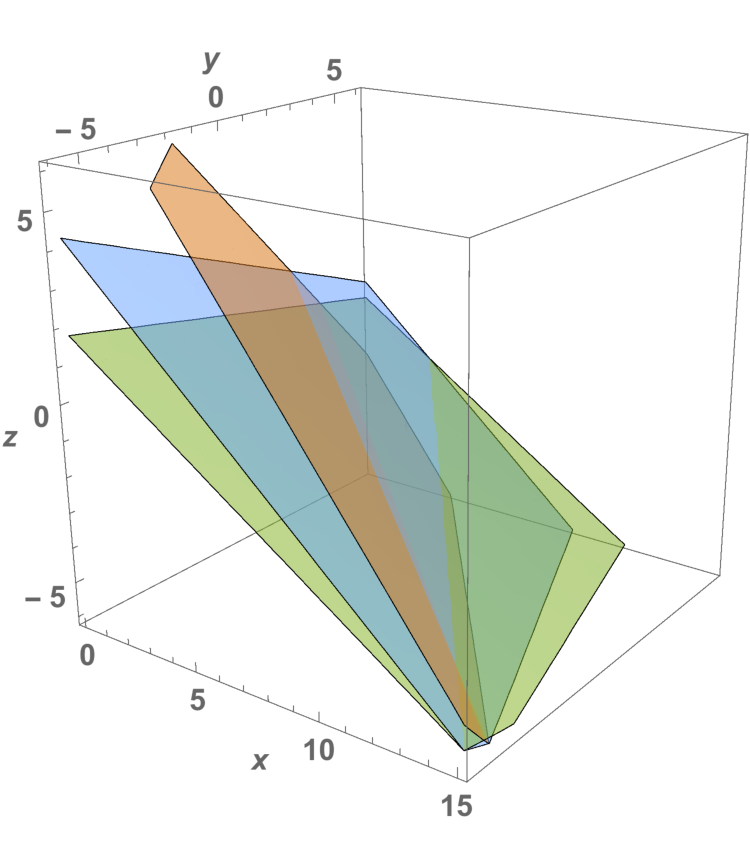
\includegraphics[width=\columnwidth]{img/LinearSystem1}
  \end{columns}
}
% 
% 
\section{Matrix inversion}
\subsection*{Inverse}
\againframe<2>{contents}

\frame{
  \frametitle{Inverse of a matrix}
  \begin{itemize}
    \item The inverse $M^{-1}$ is defined such that:
   \[ MM^{-1} = I \quad{} \text{and} \quad{} M^{-1}M=I\]
   \item Use the inverse to solve a set of linear equations:
   \begin{align*}
    M\vec{x} &= \vec{b} \\
    M^{-1}M\vec{x} &= M^{-1}\vec{b} \\
    I\vec{x} &= M^{-1}\vec{b} \\
    \vec{x} &= M^{-1}\vec{b}
   \end{align*}
  \end{itemize}
}
% 
\frame{\frametitle{How to calculate the inverse?}
  \begin{itemize}
    \item The inverse of an $N \times N$ matrix can be calculated using the co-factors of each element of the matrix:
    \[
      M^{-1} = \frac{1}{\det{M}}
      \begin{bmatrix}
      C_{11} &C_{12} &C_{13} \\
      C_{21} &C_{22} &C_{23} \\
      C_{31} &C_{32} &C_{33} \\
      \end{bmatrix}^T
    \]
    \item $\det{M}$ is the \emph{determinant} of matrix $M$.
    \item $C_{ij}$ is the \emph{co-factor} of the $ij^\text{th}$ element in $M$.
  \end{itemize}
}

\begin{frame}[fragile]
\frametitle{Computing the co-factors}
  Consider the following example matrix:
  $ M =
    \begin{bmatrix}
      1 & 1 & 1\\ 
      2 & 1 & 3\\ 
      3 & 1 & 6
    \end{bmatrix} 
  $\\ \vskip1em \pause
  A co-factor (e.g. $C_{11}$) is the \tikzmarkin[txt=style green]{det1}determinant of the elements left over\tikzmarkend{det1} when you cover up the row and column of the \tikzmarkin[txt=style cyan]{cof}element in question\tikzmarkend{cof}, \tikzmarkin[txt=style orange]{pm1}multiplied by $\pm 1$\tikzmarkend{pm1}, depending on the position. \vskip1em
  \begin{columns}
    \column{0.25\textwidth}
      \begin{equation*}
      \left[\begin{array}{ccc}
	\tikzmarkin[mat=style cyan]{col 1} 1 \tikzmarkend{col 1} &  \times & \times \\
	\times  & \tikzmarkin[mat=style green]{col 2} 1 & 3 \\
	\times  &  1   &  6 \tikzmarkend{col 2}\\
	\end{array}\right]
      \end{equation*}\pause
    \column{0.25\textwidth}
      \begin{equation*}
      \left[\begin{array}{ccc}
	\tikzmarkin[mat2=style orange]{pm} + \tikzmarkend{pm} &  - & + \\
	- & + & - \\
	+ & - & +\\
	\end{array}\right]
      \end{equation*}\pause
      \column{0.5\textwidth}
      \[ \begin{split}
C_{11} &= \tikzmarkin[mat2=style orange]{pm3}+1\tikzmarkend{pm3}\ \cdot\ \det{\begin{array}{cc}\tikzmarkin[mat=style green]{det2} 1 & 3 \\ 1 & 6\tikzmarkend{det2}\end{array}} \\
&= 6 \times 1 - 3 \times 1 = 3
\end{split}
\]
  \end{columns}
\end{frame}

\frame{\frametitle{Computing the co-factors}
    Back to our example:
    \[
      M^{-1} = \begin{bmatrix}
      1 & 1 & 1 \\
      2 & 1 & 3 \\
      3 & 1 & 6 \\
    \end{bmatrix}^{-1} = 
      \frac{1}{\det{M}}
      \begin{bmatrix}
      3 & -3 & -1 \\
      -5&  3 &  2 \\
      2 & -1 & -1 \\
      \end{bmatrix}^T
    \]\pause
    \begin{itemize}
      \item The determinant is very important
      \item If $\det{M}=0$, the inverse does not exist (singular matrix)
    \end{itemize}
}

\frame{\frametitle{Calculating the determinant}
    Compute the determinant by multiplication of each element on a row (or column) by its cofactor and adding the results:
    \[
    \det{\begin{bmatrix}
      \ \tikzmarkin[mat=style green]{horizontal}1 & 1 & 1 \tikzmarkend{horizontal}\\
      2 & 1 & 3 \\
      3 & 1 & 6 \ \end{bmatrix}} = +\det{\begin{bmatrix}1&3\\1&6\end{bmatrix}} - \det{\begin{bmatrix}2&3\\3&6\end{bmatrix}} + \det{\begin{bmatrix}2&1\\3&1\end{bmatrix}} = -1
    \]
    \pause
    \[
    \det{\begin{bmatrix}
      \ 1 & 1 & \tikzmarkin[mat=style green]{vertical}1 \\
      2 & 1 & 3 \\
      3 & 1 & 6\tikzmarkend{vertical}\ \end{bmatrix}} = +\det{\begin{bmatrix}2&1\\3&1\end{bmatrix}} - 3\det{\begin{bmatrix}1&1\\3&1\end{bmatrix}} + 6\det{\begin{bmatrix}1&1\\2&1\end{bmatrix}} = -1
    \]
}

\section{Solving a linear system}
\subsection*{Solving}
\againframe<2>{contents}

\frame{\frametitle{Solving a linear system}
  \begin{itemize}
    \item Our example:
   \[ 
      \begin{bmatrix}
	1 & 1 & 1\\ 
	2 & 1 & 3\\ 
	3 & 1 & 6
      \end{bmatrix}
      \begin{bmatrix}
	x \\
	y \\
	z 
      \end{bmatrix} = 
      \begin{bmatrix}
	4 \\
	7 \\
	5 
      \end{bmatrix} 
      \]\pause
    \item The solution is:
    \[
    \begin{bmatrix}x \\ y \\ z\end{bmatrix} = M^{-1}b= \frac{1}{-1}
    \begin{bmatrix}
      3 & -5 & 2 \\
      -3&  3 & -1 \\
      -1 & 2 & -1 \\
    \end{bmatrix} \begin{bmatrix}4 \\ 7 \\ 5\end{bmatrix} = \frac{1}{-1}\begin{bmatrix}-13 \\ 4 \\ 5\end{bmatrix} = \begin{bmatrix}13 \\ -4 \\ -5\end{bmatrix}
    \]\pause
    \item The inverse exists, because $\det{M}=-1$.
  \end{itemize}
}

\begin{frame}[fragile]
  \frametitle{Solving a linear system in Matlab using the inverse}
  \begin{itemize}
    \item Create the matrix:
    \begin{lstlisting}
>> A = [1 1 1; 2 1 3; 3 1 6];     
    \end{lstlisting}\pause
    \item Create solution vector:
    \begin{lstlisting}
>> b = [4; 7; 5]; 
    \end{lstlisting}\pause
    \item Get the matrix inverse:
    \begin{lstlisting}
>> Ainv = inv(A); 
    \end{lstlisting}\pause
    \item Compute the solution:
    \begin{lstlisting}
>> x = Ainv * b   
    \end{lstlisting}\pause
    \item Matlab's internal direct solver:
    \begin{lstlisting}
>> x = A\b
    \end{lstlisting}
    \item These are black boxes! We are going over some methods later!
  \end{itemize}
\end{frame}

\begin{frame}[fragile]
  \frametitle{Exercise: performance of inverse computation}
  Create a script that generates square matrices of various sizes $N\times N$. Computes the inverse of these matrices, and use \lstinline$tic$ and \lstinline$toc$ to see the computing time for each inversion. Plot the time as a function of the matrix size $N$. What kind of growth do you see? \pause
  \begin{lstlisting}
% Generate random matrices of various sizes 's'. 
% Invert the matrices and store the time required 
% for the inversion. Plot the times vs 's'
s = [10:10:90 100:100:1000 2000:1000:5000 10000]
for n = 1:length(s) (*@ \pause @*)
    s(n)
    A = rand(s(n)); (*@ \pause @*)
    tic;
    Ainv = inv(A);
    t_inv(n) = toc;
end
loglog(s,t_inv)
xlabel('N')
ylabel('Time [s]')
  \end{lstlisting}
\end{frame}

\begin{frame}[fragile]
  \frametitle{Exercise: sample results}
  Each computer produces slightly different results because of background tasks, different matrices, etc. This is especially noticable for small systems.
  \begin{center}
  \begin{tikzpicture}
    \begin{loglogaxis}[
      xlabel={$N$},
      ylabel={Time [s]},
%       grid = major,
      width=0.6\textwidth, height=5.5cm]
     \addplot[graph,draw=tuered,thick,mark = x] table [y index={1}] {tictocINV.dat};
     \addplot [black,very thick] table {
	900 0.065
	11000 64.87
      } coordinate [pos=0.15] (A) % save two points on the regression line for drawing the slope triangle
        coordinate [pos=0.85] (B);
	\draw[thick] (A) -| (B)  % draw the opposite and adjacent sides of the triangle
        node [pos=0.25, anchor=north] {1} % label the horizontal line
        node [pos=0.75,anchor=west] {3};
     \end{loglogaxis}
  \end{tikzpicture}
  \end{center}
  \vskip-1em
  The time increases by 3 orders of magnitude, for every magnitude in $N$. A matrix inversion scales with $\mathcal{O}(N^3)$!
\end{frame}

\begin{frame}[fragile]
  \frametitle{Solving a linear system in Excel using the inverse}\vspace{-1em}
  \[
   Ax=b \qquad \begin{bmatrix}1&1&1\\2&1&3\\3&1&6\end{bmatrix}\begin{bmatrix}x_1\\x_2\\x_3\end{bmatrix}=\begin{bmatrix}4\\7\\5\end{bmatrix}
  \]\vspace{-1em}
  \begin{itemize}
    \item Create matrix \ \tikzmarkin[mat=style green]{A}$A$\tikzmarkend{A} \ in $3\times 3$ cells
    \item Create right hand side vector \ \tikzmarkin[mat=style cyan]{b}$b$\tikzmarkend{b} \ in 3 vertical cells\pause
    \item Compute the inverse \ \tikzmarkin[mat=style orange]{I}$I$\tikzmarkend{I} \ :
    \begin{itemize}
      \item Select an empty area of $3 \times 3$ cells
      \item Type \lstinline$=MINVERSE($
      \tikzmarkin[txt=style green]{A2}\lstinline$B2:D4$\tikzmarkend{A2}
      \lstinline$)$ \footnote{In Dutch Excel: \lstinline$INVERSEMAT$}
      \item Close with Ctrl+Shift+Enter
    \end{itemize}\pause
    \item Solution:
    \begin{itemize}
      \item Select 3 vertical cells
      \item Type \lstinline$=MMULT($
      % First part, contains the inverse
      \tikzmarkin[txt=style orange]{I2}\lstinline$H2:J4$\tikzmarkend{I2}
      % Semicolon
      \lstinline$;$
      % Second part, contains the RHS
      \tikzmarkin[txt=style cyan]{b2}\lstinline$B6:B8$\tikzmarkend{b2}
      % Finish the command
      \lstinline$)$ \footnote{In Dutch Excel: \lstinline$PRODUCTMAT$. The semicolon may be a comma.}
      \item Close with Ctrl+Shift+Enter
    \end{itemize}    
  \end{itemize}
\end{frame}


\section{Towards larger systems}
\subsection*{Matrix tricks}
\againframe<2>{contents}

\begin{frame}[fragile]
  \frametitle{Towards larger systems}
  \tikz{\node[emphblock,text width=\textwidth] {Computation of determinants and inverses of large matrices in this way is too difficult (slow), so we need other methods to solve large linear systems!};}
\end{frame}

\begin{frame}[fragile]
  \frametitle{Towards larger systems}
  \begin{itemize}
    \item Determinant of upper triangular matrix:
    \[
    \det{M_\text{tri}} = \prod_{i=1}^n a_{ii} \qquad M=\begin{bmatrix}
5 & 3 & 2 \\ 
0 & 9 & 1 \\
0 & 0 & 1
\end{bmatrix} \Rightarrow \det{M} = 5 \times 9 \times 1 = 45
    \]
  \item Matrix multiplication:
  \[
  \det{AM}=\det{A}\times\det{M}
  \]
  \item When $A$ is an identity matrix ($\det{A}=1$):
  \[
   \det{AM}=\det{A}\times\det{M} = 1\times\det{M}
  \]
  \item With rules like this, we can use row-operations so that we can compute the determinant more cheaply.
  \end{itemize}
\end{frame}

\subsection*{Rank}
\begin{frame}[fragile]
  \frametitle{Solutions of linear systems}
 Rank of a matrix: the number of linearly independent columns (columns that can not be expressed as a linear combination of the other columns) of a matrix.
 \vskip1em
 \begin{columns}
  \column{0.5\textwidth}
  \[
   M = \begin{bmatrix}
        5 & 3 & 2 \\
        0 & 9 & 1 \\
        0 & 0 & 1
       \end{bmatrix}
  \]
  \begin{itemize}
   \item 3 independent columns
   \item In Matlab:
   \begin{lstlisting}
>> rank(M)
   \end{lstlisting}
  \end{itemize}
  \column{0.5\textwidth}
    \[
   M = \left[\begin{array}{cccc}
        \tikzmarkin[mat=style green]{c1}1 & \tikzmarkin[mat=style yellow]{c2}2 & \tikzmarkin[mat=style cyan]{c3}1 & \tikzmarkin[mat=style orange]{c4}0 \\
        0 & 0 & 1 & 1 \\
        0\tikzmarkend{c1} & 0\tikzmarkend{c2} & 0\tikzmarkend{c3} & 0\tikzmarkend{c4}
       \end{array}\right]
  \]
  \begin{itemize}
   \item \tikzmarkin[txt=style yellow]{c22}col 2\tikzmarkend{c22} $= 2 \times$ \tikzmarkin[txt=style green]{c12}col 1\tikzmarkend{c12}
   \item \tikzmarkin[txt=style orange]{c42}col 4\tikzmarkend{c42} $=$ \tikzmarkin[txt=style cyan]{c32}col 3\tikzmarkend{c32} $-$ \tikzmarkin[txt=style green]{c13}col 1\tikzmarkend{c13}
   \item 2 independent columns: rank = 2
  \end{itemize}
 \end{columns}
\end{frame}

\begin{frame}[fragile]
  \frametitle{Solutions of linear systems}
  The solution of a system of linear equations may or may not exist, and it may or may not be unique. Existence of solutions can be determined by comparing the rank of the Matrix $M$ with the rank of the augmented matrix $M_a$:
  \begin{lstlisting}
>> rank(A)
>> rank([A b])
  \end{lstlisting}
  Our system: $Mx = b$\\
  \[ 
    M = \begin{bmatrix}
    M_{11} & M_{12} & M_{13}\\ 
    M_{21} & M_{22} & M_{23}\\ 
    M_{31} & M_{32} & M_{33}
    \end{bmatrix} \text{,} b=\begin{bmatrix}b_1\\b_2\\b_3  \end{bmatrix} \Rightarrow 
    M_a =     \begin{bmatrix}
    M_{11} & M_{12} & M_{13} & b_1\\ 
    M_{21} & M_{22} & M_{23} & b_2\\ 
    M_{31} & M_{32} & M_{33} & b_3
    \end{bmatrix}
  \]
\end{frame}

\begin{frame}
 \frametitle{Existence of solutions for linear systems}
  For a matrix $M$ of size $n \times n$, and augmented matrix $M_a$:
 \begin{columns}
  \column{0.5\textwidth}
 \begin{itemize}
   \item $\text{Rank}(M) = n$:\\ Unique solution
 \end{itemize}
  \column{0.5\textwidth}
   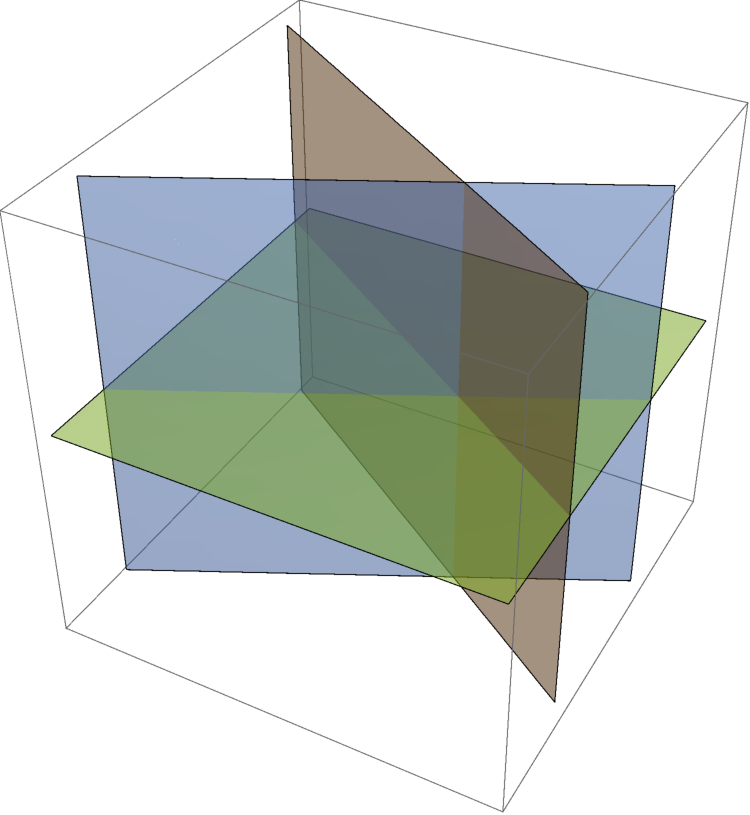
\includegraphics[width=0.4\columnwidth]{img/Rank_1-solution}
 \end{columns}
 \pause
  \begin{columns}
  \column{0.5\textwidth}
 \begin{itemize}
   \item $\text{Rank}(M) = \text{Rank}(M_a) < n$:\\ Infinite number of solutions
 \end{itemize}
  \column{0.5\textwidth}
   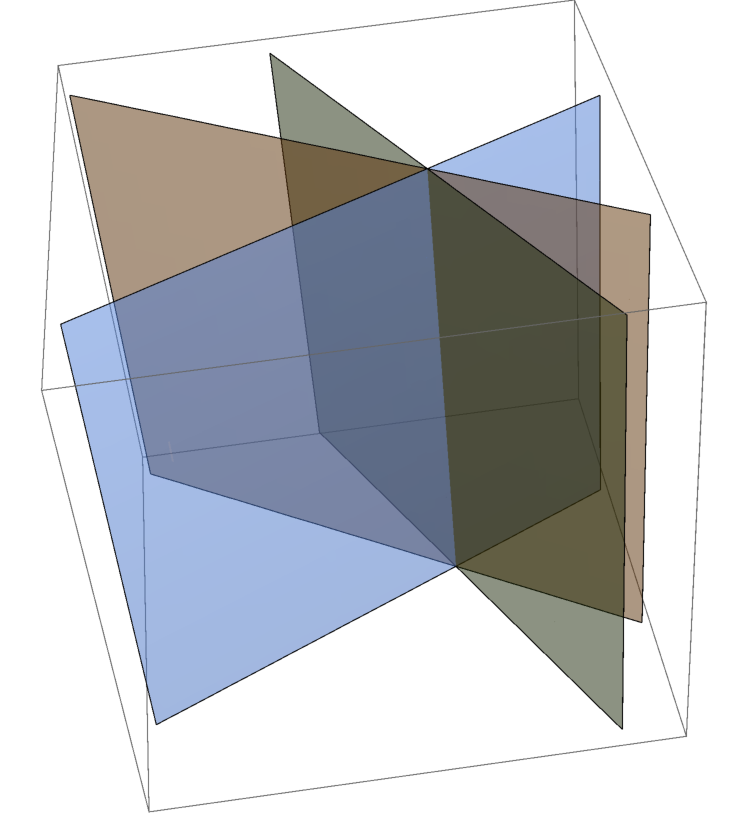
\includegraphics[width=0.4\columnwidth]{img/Rank_Inf-solutions}
 \end{columns}
 \pause
  \begin{columns}
  \column{0.5\textwidth}
 \begin{itemize}
   \item $\text{Rank}(M) < n$, $\text{Rank}(M) < \text{Rank}(M_a)$:\\ No solutions
 \end{itemize}
  \column{0.5\textwidth}
   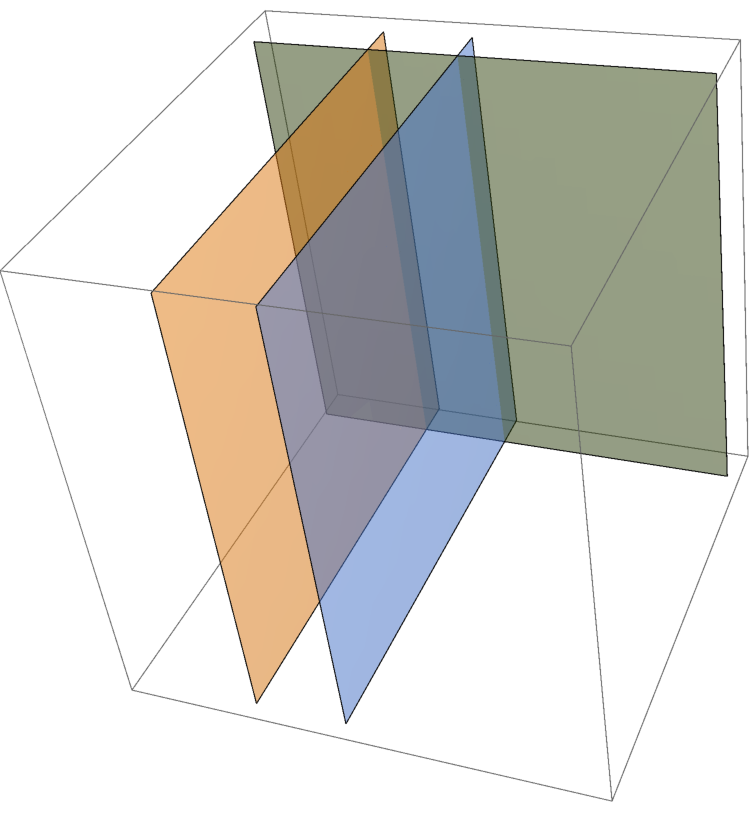
\includegraphics[width=0.4\columnwidth]{img/Rank_No-solutions1} \ \ 
   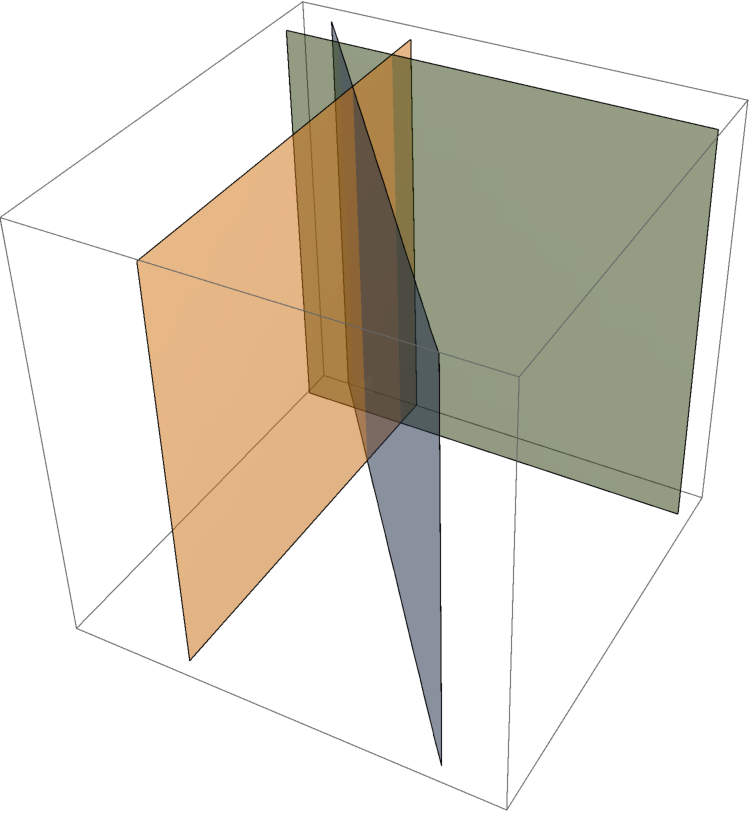
\includegraphics[width=0.4\columnwidth]{img/Rank_No-solutions2}
 \end{columns}
\end{frame}
 
\begin{frame}[fragile]
  \frametitle{Two examples}
  \[
    M=
    \begin{bmatrix}
      1 & 1 & 2\\
      0 & 3 & 1\\
      0 & 0 & 2
    \end{bmatrix}\quad
    b=
    \begin{bmatrix}
      17\\11\\4
    \end{bmatrix}
    \Rightarrow
    M_a=
    \begin{bmatrix}
      1 & 1 & 2 & 17\\
      0 & 3 & 1 & 11\\
      0 & 0 & 2 & 4
    \end{bmatrix}
  \]
  $\rank(M)=3=n \Rightarrow $ Unique solution \pause \\ \vfill
    \[
    M=
    \begin{bmatrix}
      1 & 1 & 2\\
      0 & 3 & 1\\
      0 & 0 & 0
    \end{bmatrix}\quad
    b=
    \begin{bmatrix}
      17\\11\\0
    \end{bmatrix}
    \Rightarrow
    M_a=
    \begin{bmatrix}
      1 & 1 & 2 & 17\\
      0 & 3 & 1 & 11\\
      0 & 0 & 0 & 0
    \end{bmatrix}
  \]
  $\rank(M)=\rank(M_a)=2<n \Rightarrow $ Infinite number of solutions
\end{frame} 

\section{Summary}
\subsection*{Summary}
\againframe<2>{contents}

\begin{frame}[fragile]
  \frametitle{Summary}
  \begin{itemize}
    \item Linear equations can be written as matrices
    \item Using the inverse, the solution can be determined
    \begin{itemize}
      \item Inverse via cofactors
      \item Inverse and solution in Matlab
      \item Inverse and solution in Excel
    \end{itemize}
    \item Inversion scales with $N^3$
    \item A solution depends on the rank of a matrix
  \end{itemize}
\end{frame}
\end{document}
